\chapter{Related Work}

Global illumination is a broad topic that can be approached in many ways. With respect to this thesis, we only focus on comparisons with other real-time, fully dynamic techniques. Many of these techniques borrow similar ideas and build off of each other. The implementations for a single technique can also vary greatly based on data structures used, shading models, and other considerations. The different tradeoffs made and how they affect the final implementation are important to understand, as there is often not a single best way to approach the problem of global illumination. Here we present some of the more popular and relevant methods of achieving full global illumination and attempt to note the major differences between them and our implementation.

\section{Reflective Shadow Maps}
Dachsbacher and Stamminger introduced the idea of Reflective Shadow Maps (RSMs) in 2005~\cite{Dachsbacher:2005:RSM:1053427.1053460}. Their work extends traditional shadow mapping to support single bounce indirect illumination. The main idea is to treat each pixel in the shadow map as a virtual point light (VPL)---i.e., each pixel in the shadow map corresponds to a directly lit point---which illuminates the rest of the scene\footnote{VPLs were introduced in Keller's work on Instant Radiosity~\cite{Keller:1997:IR:258734.258769}.}. The information gathered for each reflective shadow map is shown in Figure~\ref{fig:rsm}. In order to efficiently compute the contribution of the VPLs for a point in the scene a fixed number of samples are taken from the shadow map. They also apply an interpolation scheme to reduce computation on smooth parts of the scene.

\begin{figure}[h]
    \centering
    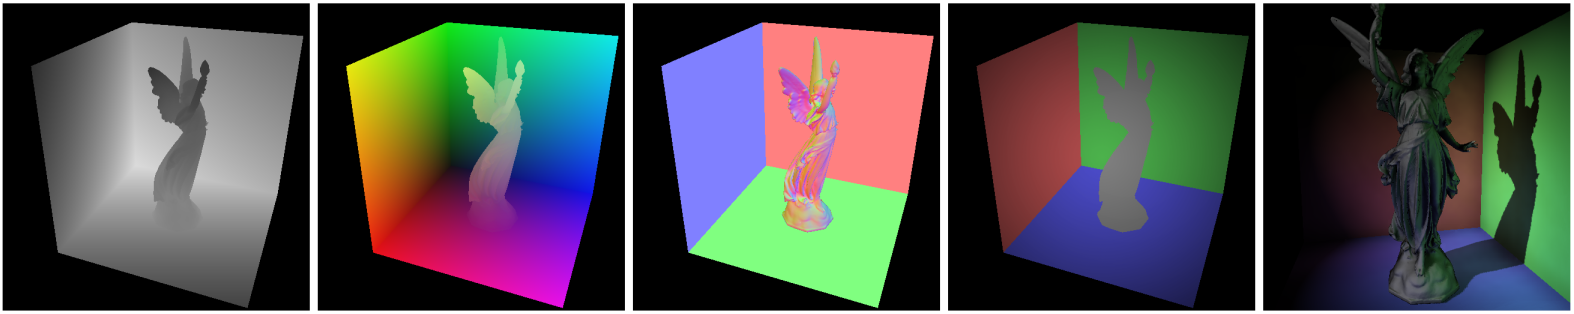
\includegraphics[scale=0.25]{rsm.png}
    \caption{The different components of a reflective shadow map (depth, world coordinates, normal, and color) and the resulting image~\cite{Dachsbacher:2005:RSM:1053427.1053460}.}
    \label{fig:rsm}
\end{figure}

A notable downside of this method is occlusion information is not accounted for: a point $y$ could contribute indirect lighting to another point $x$ even if there is other geometry blocking the path between $x$ and $y$. The authors apply a separate ambient occlusion pass to partially mitigate this problem. The method is also only designed for low frequency lighting details. Also, while directional, point, and spot lights should theoretically work, objects that themselves emit light were not addressed.

\section{Cascaded Light Propagation Volumes}
Light Propagation Volumes (LPVs) are another method for approximating low frequency indirect lighting, developed by Kaplanyan and Dachsbacher in 2010~\cite{Kaplanyan:2010:CLP:1730804.1730821}. The method relies on an iterative based light propagation algorithm within a volumetric grid structure. This structure, the LPV, is initialized by injecting VPLs into its cells---for example, by using RSMs. Next, the light is propagated multiple times between adjacent cells; each propagation results in the LPV having a more complete representation of the indirect light in the scene.

LPVs improve on the basic RSM idea by filtering the light in multiple steps. It also stores low resolution geometry information for occlusion purposes. They also tackle the issue of handling large scenes with the concept of cascaded LPVs: multiple individual LPV structures are used with different sizes, focusing detail near the camera (shown in Figure~\ref{fig:lpv}).

\begin{figure}[h]
    \centering
    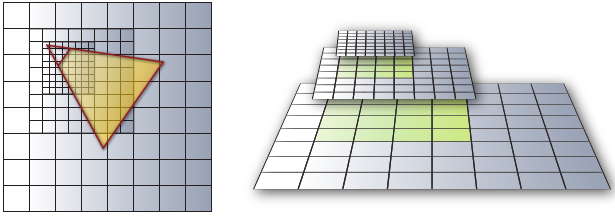
\includegraphics[scale=0.5]{lpv.png}
    \caption{A diagram demonstrating the grids used for cascaded LPVs~\cite{Kaplanyan:2010:CLP:1730804.1730821}.}
    \label{fig:lpv}
\end{figure}

% TODO do authors mention performance or memory cost of adding their improvements?
The main drawback of this method is the lighting is low frequency only. Proper glossy (specular) reflections are still wanted in many applications. Also, the geometry information obtained is not complete: it is created by reusing other results from shadow mapping and depth peeling.

% TODO refer to citations as nouns?
\section{Rasterized Voxel-Based Dynamic Global Illumination}
Rasterized Voxel-Based Dynamic Global Illumination described by Doghramachi~\cite{doghramachi2013rasterized} is based heavily on LPVs but uses a voxelized scene representation for the initial steps of LPV creation. This avoids some of the difficulties when injecting VPLs compared to LPVs. In addition, the geometry information made available by voxelization is complete (although low-resolution) and does not require external inputs like shadow maps or depth peeling.

Just like LPVs, the main downside here is the lack of specular reflections, which stems from the low resolution grid used for the LPV (32x32x32, as mentioned in the implementation, whereas we aim for somewhere on the order of $128^3$ to $256^3$). Also, the method does suffer from some light leaking due to how point lights are injected into the scene: instead of creating an RSM (which handles occlusion properly), all voxels within a defined distance of the point light are injected into the initial LPV.

\section{Voxel Cone Tracing}
In 2011, Crassin et al.\ introduced Interactive Indirect Illumination Using Voxel Cone Tracing~\cite{crassin2011interactive}. A primary improvement over the existing methods sought in this method was to obtain higher frequency lighting details, such as specular reflections. The core idea to balance performance with lighting detail is to make use of a filtered radiance representation which is then sampled using voxel cone tracing, a concept they introduce.

The first step in the algorithm is to create a high resolution radiance representation. Crassin et al.\ inject radiance into the leaves of an octree using the familiar RSM technique. An octree is used to reduce memory consumption, a consequence of using such a high resolution radiance representation. The octree is then filtered recursively bottom up until all inner nodes in the octree have a filtered radiance value. The final step, voxel cone tracing, is essentially a combination of raymarching and mipmapping: raymarched samples are taken from successively lower levels of detail. An illustration of this is shown in Figure~\ref{fig:vct}.

% TODO move the section on vct from implementation here instead?
% TODO by varying the angle of the cone, different affects can be replicated: large -> diffuse, small -> specular

Although the octree representation does help alleviate issues when dealing with sparse scenes, GPU memory consumption is still an issue especially for larger scenes. In addition, due to their tree-like nature, octrees are awkward for GPU use and do not benefit from things like hardware supported texture filtering. To address this, NVIDIA decided to use a clipmap instead of an octree in their standard implementation of voxel cone tracing, VXGI~\cite{nvidiavxgi}.

\begin{figure}[h]
    \centering
    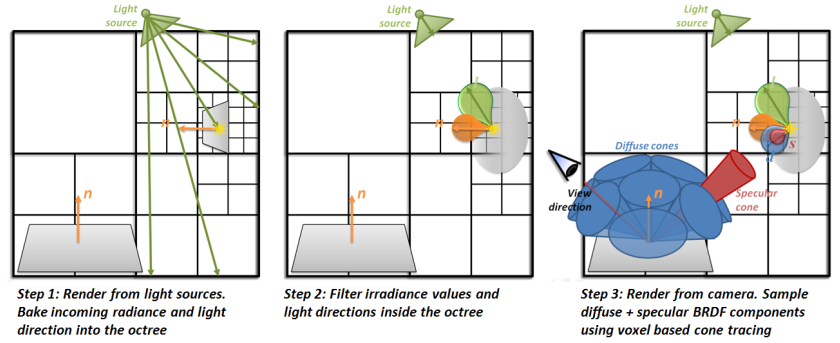
\includegraphics[scale=0.5]{vct.png}
    \caption{An illustration of the voxel cone tracing algorithm by Crassin et al.~\cite{crassin2011interactive}.}
    \label{fig:vct}
\end{figure}

% TODO explain why warping may be better approach: simpler (one texture), memory use, easily configurable, better suited to large scenes?

% TODO image-space approaches: incomplete scene info
